\documentclass[../main.tex]{subfiles}

\begin{document}

\chapter{Validation of TF-promoter interactions}\label{chapter4}
\section{Introduction}\label{chapter4:introduction}
Recently, systems biology approaches have identified a nitrogen response subnetwork \autocite{gaudinierTranscriptionalRegulationNitrogenassociated2018}.
This is composed of many network motifs such as feed forward loops (FFLs).
%Add figure of network and subnetwork
We would like to validate the subnetwork to characterise the role of network components and their connections (edges) so that they can be rationally and predictably engineered.
Yeast one-hybrid and DAP-seq experimental techniques suggest hypotheses for edges but they are not definitive as they do not determine whether edges activate or repress their target genes.
We are using an in-house method called TRAMP to quantitatively determine TF-DNA binding affinity (lab work done by Yaomin Cai).
We are also using the TARGET method to determine direct and indirect targets of TFs~\autocite{bargmannTARGETTransientTransformation2013}.
Using TRAMP and TARGET assays we would like to validate edges in the nitrogen response network.
\section{Aims}\label{chapter4:aims}
To validate edges in the N-response GRN and test whether they activate or repress their targets using TARGET~\autocite{bargmannTARGETTransientTransformation2013}.
To validate the binding affinity of N-reponse TFs to their proposed TFBS in promoters of their targets using the TRAMP assay.
\section{Results}\label{chapter4:results}
The binding affinity of TGA1, NLP7 and NLP6 to promoters in the N subnetwork has been measured using TRAMP and EMSA (\autoref{fig:tramp}).
\begin{figure}[hbt!]
	\begin{center}
		\capstart
		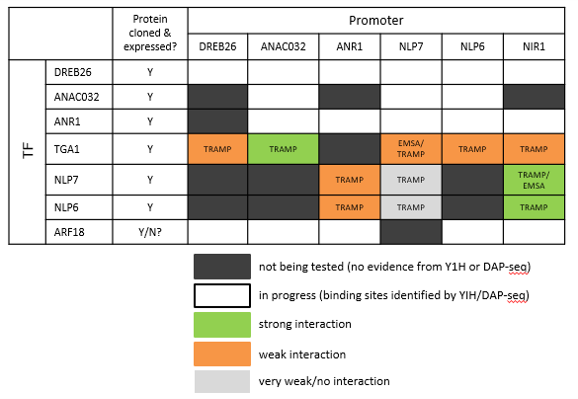
\includegraphics[width=0.60\columnwidth]{validate_edges/TRAMP}
		\caption{
			\textbf{In vitro validation of TF-promoter interactions using ElectroMobility Shift Assay (EMSA) and/or Transcription-factor Relative binding Affinity Measurement Platform (TRAMP)}
			TFs were expressed and their binding affinity to promoters of important master regulators was measured using TRAMP and in some cases EMSA.
            This was to validate predicted yeast one\hyp{}hybrid (Y1H) \autocite{gaudinierTranscriptionalRegulationNitrogenassociated2018} and DNA affinity purification sequencing {DAP-seq} \autocite{omalleyCistromeEpicistromeFeatures2016} edges in the N \hyp{}response subnetwork.
			\label{fig:tramp}
		}
	\end{center}
\end{figure}

Tufan Oz and I set up the TARGET~\autocite{bargmannTARGETTransientTransformation2013} method in the lab to determine direct and indirect targets of nodes and whether they activate or repress each target.
Since setting up the protocol, Tufan has validated the direct and indirect targets of NLP7 using TARGET and qPCR.
(I will include results here in my thesis)

\section{Discussion}\label{chapter4:discussion}

\end{document}